\chapter{Le caratteristiche dell'OnBoarding}\label{chapter:caratteristiche_onboarding}
Il processo di OnBoarding, sebbene possa inizialmente apparire come una fase apparentemente semplice e marginale, 
riveste in realtà un'importanza cruciale nel contesto dell'integrazione dei nuovi membri nell'organico di ISolutions.\
Come precedentemente introdotto nella sezione iniziale di questo elaborato~\ref{chapter:introduzione}, %TODO fixhere
il processo di OnBoarding è tipicamente strutturato su un periodo di circa un mese, ma è fondamentale sottolineare che 
la sua durata può variare considerevolmente da un dipendente all'altro.\ Questo periodo iniziale di integrazione, 
che potrebbe superficialmente sembrare un'appendice, svolge in realtà una serie di funzioni di rilevanza vitale.
\\ \\
È importante notare che il processo di OnBoarding viene coordinato e gestito con grande cura da un team HR altamente specializzato.\ 
Questo team opera con precisione e attenzione ai dettagli per garantire una transizione efficace e senza intoppi per i nuovi arrivati.\ 
La sua importanza ricade con lo scopo di offrire una garanzia di un'ottimale integrazione dei nuovi dipendenti nell'ambiente aziendale.
\\ \\
Risulta evidente che il processo di OnBoarding richiede un approccio attento e uniforme da parte di tutto il personale aziendale.\ 
Questa necessità è strettamente correlata alla complessità delle operazioni svolte da ISolutions e alla diversità dei numerosi 
strumenti e tecnologie che l'azienda utilizza, compresi quelli di natura proprietaria.\ Questi strumenti rivestono un ruolo 
centrale sia nella gestione che nell'analisi dei dati aziendali e nei processi operativi nel loro complesso.\ 
Inoltre, essi giocano un ruolo significativo nella consegna di servizi di alta qualità ai clienti dell'azienda.
\\ \\
In questo contesto, diventa chiaro che un nuovo membro del team deve affrontare l'obiettivo di familiarizzarsi 
con tali tecnologie e procedure aziendali.\ Questo obiettivo viene raggiunto attraverso il processo di OnBoarding, 
che svolge il ruolo di guida nella presentazione di tutte le conoscenze iniziali necessarie per lavorare in modo produttivo 
all'interno del sistema aziendale. Durante questa fase, i nuovi arrivati avranno l'opportunità di acquisire familiarità con 
gli strumenti, i linguaggi, le convenzioni aziendali e i protocolli che sono essenziali per contribuire al successo e 
all'efficienza dell'azienda.
\\ \\
Pertanto, il processo di OnBoarding, lungi dall'essere una mera formalità, rappresenta un elemento fondamentale per il successo 
e il corretto funzionamento di ISolutions e deve essere affrontato con la massima serietà e impegno da parte di tutti i suoi attori.
\\ \\
Il processo di OnBoarding è un'attività complessa che si pone diversi obiettivi, 
e pertanto è strutturato in diverse sezioni con l'intento di fornire ai nuovi 
dipendenti una conoscenza iniziale completa.\ Le sezioni principali del processo di OnBoarding si suddividono in:
%TODO aggiungere le varie categorie e descriverle
\begin{itemize}
    \item Video;
    \item Documentazione;
    \item Hands On;
    \item Audit;
\end{itemize}
%
Al momento, come precedentemente accennato, il processo di OnBoarding non fa uso di un sistema automatizzato; 
al contrario, è gestito attraverso un semplice foglio Excel. Questo foglio è consultato dai dipendenti interessati 
e viene modificato manualmente quando il dipendente termina le relative attività interne da parte del personale HR incaricato.\ 
Tuttavia, questo approccio presenta alcune limitazioni.\ 
Innanzitutto, non permette di raccogliere e organizzare dati statistici derivati dall'uso del processo.\ 
In secondo luogo, non offre la possibilità agli utenti di interagire direttamente con il sistema.
\\ \\
Ciò significa che, con l'attuale modalità, manca l'opportunità di ottenere una visione dettagliata e sistematica dell'andamento del processo di OnBoarding, 
impedendo all'azienda di identificare potenziali aree di miglioramento o di misurare l'efficacia del processo stesso.\ 
Inoltre, l'assenza di un'interazione diretta con il sistema può ostacolare la comunicazione e la partecipazione attiva dei dipendenti nel corso 
del processo, rendendo l'integrazione meno fluida e coinvolgente.
\\ \\
Pertanto, esiste un evidente margine per l'implementazione di un sistema automatizzato di OnBoarding che non solo semplificherebbe 
la gestione, ma consentirebbe anche la raccolta e l'analisi di dati utili per ottimizzare il processo e coinvolgere in modo più 
attivo i dipendenti coinvolti.
%TODO inserire immagine esempio di un template del processo di onboarding
% \begin{figure}[ht]
% 	\centering
% 	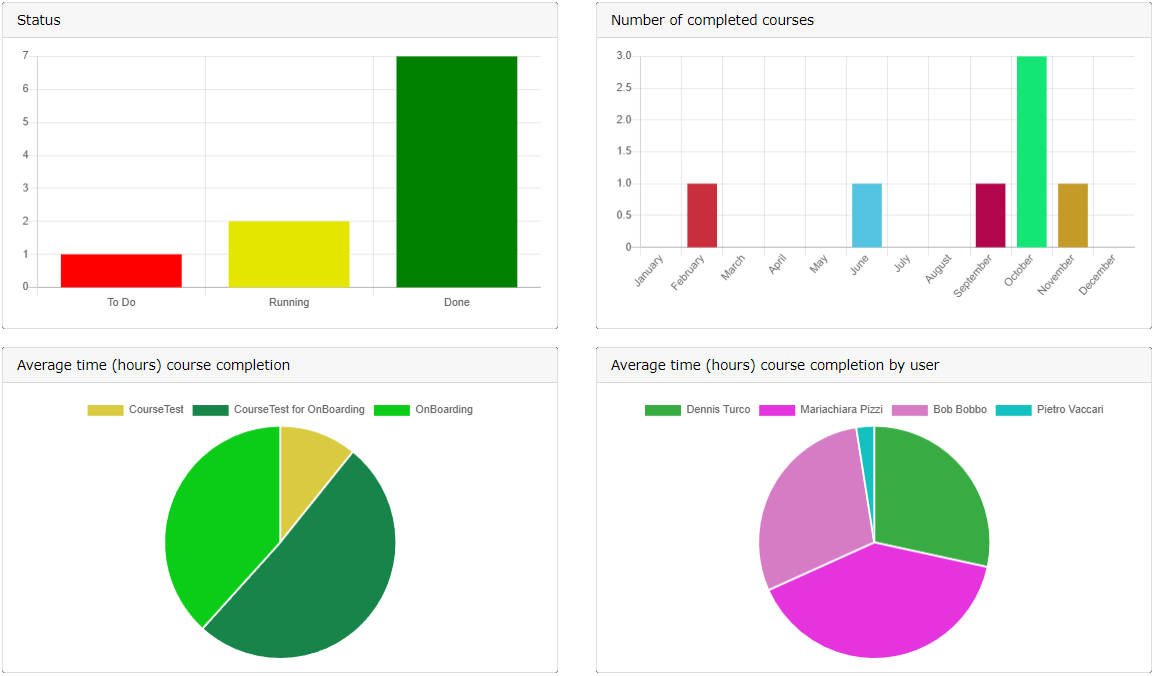
\includegraphics[width=0.7\textwidth]{img/charts.png}
% 	\caption{struttura del file excel di OnBoarding}
% 	\label{fig:charts}
% \end{figure}